%% Quadratic Volumes
%% File Created 3/22/07.

\section{Properties of Measure}

Nowhere in the proof of the Kepler conjecture do we need a notion
of integration.  Measure alone suffices.  (However, there are a few
volumes described below that I do not see how to calculate without
first writing them as an integral.)

We need a concepts of null set, measurable set, and volume in
three dimensions.  For the purposes of this paper, we can take the
the three dimensional Lebesgue measure.   
The null sets can be defined
to be the sets of zero Lebesgue measure. The measurable sets can
be defined as the bounded Lebesgue measurable sets.  The volume of
a measurable set can be defined as its Lebesgue measure.

As we will see in a moment, we need considerably less than this.
We could, for instance,
take measurable to mean Jordan measurable.   We could define
measure to mean Jordan measure.  We could define null sets to be
finite unions of planes, spheres, and cones.



\subsection{properties of null sets}

We assume that have the following
properties.

\begin{enumerate}%[Null Set]
\label{enum:null}
\item A finite union of null sets is a null set.\\
 \item A plane is a null set.\\
 \item A sphere is a null set.\\
 \item A circular cone is a null set; that is, a union of all
  lines through a fixed point $P$ and forming fixed
 forming fixed angle with a line through $P$.
\end{enumerate}

We write $A\equiv B$ if sets $A$ and $B$ are equal up to a null set.
That is, there exists a null set $E$ such that
   $(A\setminus B) \cup (B\setminus A) \subset E$.
\index{null set}\index{ZZZequiv@$\equiv$}

\subsection{properties of measurability}

\begin{enumerate}%[Measurable set]
\label{enum:measure}
 \item The union of two measurable sets is measurable.\\
 \item The intersection of two measurable sets is measurable.\\
 \item The difference of two measurable sets is measurable.
\end{enumerate}

\subsection{properties of volume}

\begin{enumerate}%[Volume]
\label{enum:volume}
 \item The volume is defined for every measurable set.  It is
    a non-negative real number.
 \item If $X$ and $Y$ are  measurable, and if
 the symmetric difference of
 $X$ and $Y$ is contained in a null set, then 
    $X$ and $Y$ have the same volume.\\
 \item If $X$ and $Y$ are measurable sets, and if $X\cap
 Y$ is contained in a null set, then
    $$
    \op{vol}(X\cup Y) = \op{vol}(X) + \op{vol}(Y).
    $$
  \item (linear stretch) If $X\subset \ring{R}^3$, $t\in\ring{R}$, 
    $i=1,2,3$, and $e_i\in\ring{R}^3$ is the $i$th standard basis vector,
    set 
      $$T_i(X,t) = \{ u + (t-1) u_i e_i \mid u\in X\}.
      $$
    If $X$ is measurable, then $X'=T_i(X,t)$ is as well,
    and $\op{vol}(X') = |t|\op{vol}(X)$.
  \item (translation) If $X\subset \ring{R}^3$ and $v\in\ring{R}^3$, then let
    $X+v = \{x + v\mid x\in X\}$.  If $X$ is measurable, then $X+v$ is
    as well, and $\op{vol}(X) = \op{vol}(X+v)$.
\end{enumerate}

In particular, if $X$ is contained in a null set, we may take
$X=Y$ in the preceding to deduce that $\op{vol}(X)=0$.

In addition to these properties, we will also need specific
volume calculations of primitive regions as described in
Lemmas~\ref{lemma:prim-volume} and~\ref{lemma:wedge-vol}.
%% NB Don't need lemma:wedge-sol because solid of a FR is a SC.
%% Don't need lemma:prim-sol, because solds are SC or ST.

\subsection{radial sets and solid angle}

As mentioned in the introduction, it is possible to eliminate all
surface integrals by replacing them by volumes.  The most
important case of this is the surface area that goes by the name
`solid angle.'  This gives a definition of solid angle as a
volume.


\begin{definition}
    A set $C$ is $r$-radial at center $x$ if  $C\subset B(x,r)$
    and if
        $x + u \in C$ implies
        $x + t u \in C$ for all $t$ satisfying $0\le |u| t < r$.
A set $C$ is eventually radial at center $x$ if $C\cap B(x,r)$ is
$r$-radial at center $x$, for some $r>0$.
\end{definition}

\begin{lemma}\label{lemma:r-r'}
Assume that $C$ is measurable and $r$-radial at $x$.  Let $0\le r'<r$,
then $C\cap B(x,r')$ is measurable and
$\op{vol}(C\cap B(x,r')) = \op{vol}(C) (r'/r)^3$.
\end{lemma}

\begin{proof}  We can transform $C$ into $C\cap B(x,r')$ by
a series of translations and stretch transformations.
\end{proof}


\begin{definition}
If $C$ is measurable and eventually radial at center $x$, then we
define the solid angle of $C$ at $x$ to be
    $$
    \op{sol}(x,C) = 3 \op{vol}(C\cap B(x,r))/r^3,
    $$
where $r$ is as in the definition of eventually radial. 
By Lemma~\ref{lemma:r-r'}, this
definition is independent of any such $r$.  When the center $x$ is
clear from the context, we write $\op{sol}(C)$ for
$\op{sol}(x,C)$.
\end{definition}



The following properties follow immediately from the definitions.
If $C$ is $r$-radial for some $r>0$ then it is eventually radial.
If $C$ is measurable and $r$-radial, then the volume of $C$
satisfies
    $$
    \op{vol}(C) = \op{sol}(C) r^3/3.
    $$
If $C$ is bounded away from $x$, then $C$ is eventually radial at
$x$, and $\op{sol}(C) = 0$.








\section{Primitive Volumes}

There are only a few primitive volumes that will be needed.  All
other volumes that we need will be obtained from these with
Hilbert style scissor and congruence operations.  In this sense,
our discussion is hardly about measure at all.  The focus is rather on
the geometry of the various regions and how to decompose them into
primitives.

We prefer to take the volume of open sets whenever that can be
arranged.  We begin with a description of some of the primitive
regions.






\subsection{ball}

\begin{definition}  The open ball $B(x,r)$ with center $x$ and
radius $r$ is the set
    $$
    \{ y\in\ring{R}^3 \mid |x-y| < r.\}
    $$
\end{definition}


\subsection{lune}

The set $\op{aff}^0_+(\{v_0,v_1\},\{v_2,v_3\})$ was defined
in Definition~\ref{def:aff}.  We call it a lune.  It is the intersection
of two open half-spaces
    $$
    \op{aff}^0_+(\{v_0,v_1,v_2\},v_3)\cap
    \op{aff}^0_+(\{v_0,v_1,v_3\},v_2)
    $$


\subsection{solid triangle}

\begin{definition} The solid triangle $ST(v_0,\{v_1,v_2,v_3\},r)$ is
specified by four points $v_i\in\ring{R}^3$, and a radius $r\ge0$. 
    $$
    ST(v_0,\{v_1,v_2,v_3\},r) = 
    B(v_0,r)\cap \op{cone}(v_0,\{v_1,v_2,v_3\}).
    $$
\end{definition}



\subsection{conic cap}

% renamed from spherical cap.

\begin{definition}
The conic cap $SC(v_0,v_1,r,a)$ is specified by an apex
$v_0\in\ring{R}^3$, a radius $r\ge0$, a non-zero vector $v_1-v_0$ giving
direction, and constant $a$.  The conic cap is the intersection of
the ball $B(v_0,r)$ with a solid right-circular cone:
    $$
    \{y \in B(v_0,r) \mid (y-v_0)\cdot (v_1-v_0) > |y-v_0|\, |v_1-v_0|\, a\}.
    $$
\end{definition}

\subsection{frustum}

\begin{definition} The frustum
$FR(v_0,v_1,h',h,a)$ is specified by an apex $v_0\in\ring{R}^3$, heights
$0\le h'\le h$, a vector $v_1-v_0$ giving its direction, and
$a\in[0,1]$. The set $FR$ is given as
    $$
    \{ y \mid (y-v_0)\cdot (v_1-v_0) > |y-v_0| |v_1-v_0|  a \ \ \land\ \
       h'|v_1-v_0| < (y-v_0) \cdot (v_1-v_0) < h|v_1-v_0| \}.
    $$
\end{definition}

When $h'=0$, the frustum extends to the apex, and
we write $FR(v_0,v_1,h,a)=FR(v_0,v_1,h',h,a)$.

\subsection{tetrahedron}

\begin{definition} A tetrahedron is a set of the form
$$\op{conv}^0\{v_1,v_2,v_3,v_4\}.$$
\end{definition}

By Lemma~\ref{tarski:hedra-tope}, this set can also be described
as the intersection of four open half-spaces, with each bounding
plane defined by three of the four points.
Taking this into account,
these sets can all be defined by linear and quadratic
constraints.

\subsection{primitive}

\begin{definition} A primitive region is any of the following.

\begin{enumerate}%%[Primitive Volumes]
\label{enum:volume-prim}
 \item A solid triangle $ST$.
 \item A tetrahedron $S$.
 \item A wedge of a frustum (with $h'=0$); 
that is, the intersection of a frustum with
 a lune:
    $$
     FR(v_0,v_1,h,a) \cap \op{aff}^0_+(\{v_0,v_1\},\{v_2,v_3\}).
    $$
\item A wedge of a conic cap; that is, the intersection of a conic cap
with
    a lune:
    $$
    SC(v_0,v_1,r,c) \cap\op{aff}^0_+(\{v_0,v_1\},\{v_2,v_3\}).
    $$
\end{enumerate}

\end{definition}

\subsection{primitive volume calculation}

\begin{lemma}\label{lemma:prim-volume} 
\begin{enumerate} 
 \item Let $v_1,v_2,v_3$ be unit vectors.
   A solid triangle $ST(v_0,\{v_1,v_2,v_3\},r)$ has volume
   $$
   (\alpha_{123}+\alpha_{231}+\alpha_{312}-\pi)r^3/3,
   $$
   where $\alpha_{ijk} = \dih_V(\{v_0,v_i\},\{v_j,v_k\})$.
  \item The conic cap $SC(v_0,v_1,r,a)$ has volume:
   $$
    2\pi(1-a) r^3/3,
   $$
 \item A frustum $FR(v_0,v_1,h,a)$ has volume:
   $$
   \pi (t^2-h^2) h/3,\quad h = t a.
   $$
 \item A tetrahedron $\op{conv}^0(\{v_1,v_2,v_3,v_4\})$ has volume:
   $$
   \sqrt{\Delta(x_{12},x_{13},x_{14},x_{34},x_{24},x_{23})}/12,
   $$
   where $x_{ij} = |v_i-v_j|^2$.
\end{enumerate}
\end{lemma}

Euler formula (Lemma~\ref{lemma:euler}) gives an
equivalent expression for $(\alpha_{123}+\alpha_{231}+\alpha_{312}-\pi)$.
Euler's formula will often be used instead of this formula.

\begin{proof}
The formula for the volume of a solid triangle is $r^3/3$ times
its solid angle.  The formula 
   $$\alpha_{123}+\alpha_{231}+\alpha_{312}-\pi$$
for the area of a spherical triangle is due to T. Harriot.  A
simple
derivation based on the solid angle of a lune
is found in \cite{EZ}.  The conic cap volume is
$r^3/3$ times its solid angle.  The solid angle is a simple
integral that yields the solution to Tarski's Plank Problem
\cite{EZ}.
The volume of a right-circular cone is $1/3$ its base times height.
The volume of a tetrahedron is
   $$|\det(v_2-v_1,v_3-v_1,v_4-v_1)|/6.$$
By Cayley-Menger, the square of this determinant is given by a formula
$\op{CM}_4(x_{ij})$, which by Lemma~\ref{tarski:cm4} is
$\Delta/4$, with $\Delta\ge0$.  The result follows.
\end{proof}



\subsection{wedge}

If the region is realized by revolution along an axis $\op{aff}\{v_0,v_1\}$, 
then
we can also give the volume of the intersection of the region
with a lune $A=\op{aff}^0_+(\{v_0,v_1\},\{v_2,v_3\})$.  In the following
let $\theta = \dih_V(\{v_0,v_1\},\{v_2,v_3\})$.


\begin{lemma}\label{lemma:wedge-vol}  Let $C$ be either $SC(v_0,v_1,r,a)$ or
   $FR(v_0,v_1,h,a)$.  Let $m$ be the volume of $C$.  
   Then $C\cap A$ has volume $m\,\theta/(2\pi)$.   
\end{lemma}

\begin{lemma}\label{lemma:wedge-sol}  Let $C$ be either $SC(v_0,v_1,r,a)$ or
   $FR(v_0,v_1,h,a)$.  Then $C$ is eventually radial.  Let
   $s$ be the solid angle of $C$.  Then
    $C\cap A$ is eventually radial and has solid angle 
  $s\,\theta/(2\pi)$.
\end{lemma}


\begin{proof}
These are elementary integrals.
\end{proof}


\subsection{radial}

All of the primitive sets are eventually radial, so we may take their
solid angle.  By Lemma~\ref{lemma:wedge-sol}, it is enough to compute
the solid angle before intersecting with a lune.

\begin{lemma} \label{lemma:prim-sol}
\begin{enumerate}
    \item  $ST(v_0,\{v_1,v_2,v_3\})$ is eventually radial at $v_0$
     with solid angle 
     $$
     (\alpha_{123}+\alpha_{231}+\alpha_{312}-\pi),\quad
     \alpha_{ijk}=\dih_V(\{v_0,v_i\},\{v_j,v_k\}).
     $$
    \item $SC(v_0,v_1,r,a)$ is eventually radial at $v_0$ with solid
      angle 
      $2\pi(1-a)$.
    \item $FR(v_0,v_1,h,a)$ is eventually radial at $v_0$ with solid
      angle
        $$
        2\pi (1-a).
        $$
    \item $\op{conv}^0\{v_0,v_1,v_2,v_3\}$ is eventually radial at $v_0$
      with solid angle
           $$
     (\alpha_{123}+\alpha_{231}+\alpha_{312}-\pi),\quad
     \alpha_{ijk}=\dih_V(\{v_0,v_i\},\{v_j,v_k\}).
     $$
\end{enumerate}
\end{lemma}

\begin{proof} In every case, the intersection of 
  the region with $B(v_0,r')$, for $r'>0$ sufficiently small, is
  a conic cap or a solid triangle.  These two volumes have
  already been calculated.  This gives the results as stated.
\end{proof}

\section{Scissors and Volumes}
\label{sec:measure_second}

There are many other volumes that can be computed from the
primitive ones enumerated in Definition~\ref{enum:volume-prim}.

\subsection{lune}  

To give a simple example of a derived volume, we consider the
lune $A=\op{aff}_+^0(\{v_0,v_1\},\{v_2,v_3\})$.  It is eventually
radial at $v_0$, so we may compute its solid angle.

Let $B_{\pm} = \op{aff}_+(\{v_0,v_2,v_3\},v_1)$.  $B_- \cap B_+$
is a null set.  The intersections $A\cap B_{\pm}\cap B(v_0,r)$ 
are solid triangles.  This gives the solid angle of $A$ as
follows:
   $$\begin{array}{lll}
   \sol(v_0,A) &= \sol(v_0,A\cap B_+)+\sol(v_0,A\cap B_-) \\
   &= 
   \sol(ST(v_0,\{v_1,v_2,v_3\})) + \sol(ST(v_0,\{v_1',v_2,v_3\})) \\
   &=
   2\dih_V(\{v_0,v_1\},\{v_2,v_3\}).
   \end{array}
   $$
Here, we have used $v_1'= 2 v_0 - v_1$, the reflection of $v_1$
through $v_0$.    

(The usual calculation of the volume of a solid triangle
inverts this, and derives the volume from the solid angle of a lune.)

Similarly, the ball is the union of eight quadrants, each of
which is a solid triangle whose volume is given in
 Lemma~\ref{lemma:prim-volume} as $\pi r^3/6$. It follows that
a ball of radius $r$ has volume $4\pi r^3/3$ and solid angle
$4\pi$.



\subsection{Rogers simplex}

\begin{definition} \label{def:ortho}
An {\it orthosimplex} is a tetrahedron
    $$\op{conv}^0(x,x+v_1,x+v_1+v_2,x+v_1+v_2+v_3),$$
where $v_i\cdot v_j=0$, for $1\le i<j\le 3$.   We write
$\op{orth}^0(x,v_1,v_2,v_3)$ for this orthosimplex.
 \index{orthosimplex}
\end{definition}

\begin{figure}[htb]
  \centering
  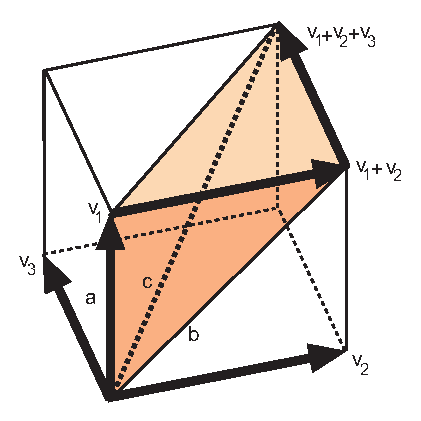
\includegraphics{\ps/rogers.eps}
  \caption{The Rogers simplex is an orthosimplex.}
  \label{fig:rogers}
\end{figure}


\begin{definition} \label{def:rog}
Let $\{v_0,v_1,v_2,v_3\}$ be a set of four points in $\ring{R}^3$.
Assume that they are not coplanar.  Let $p$ be the circumcenter
of $\{v_0,v_1,v_2\}$ and $\eta$ its circumradius.  Let $c\ge r$.
By Lemma~\ref{tarski:rog-exist}, there exists a unique
point $p'$ in $A=\op{aff}_+(\{v_0,v_1,v_2\},v_3)$ at equal distance $c$
from $v_0,v_1,v_2$.
Let $$
    \op{rog}^0(v_0,v_1,v_2,v_3,c) = 
    \op{ortho}^0(v_0,w_1,w_2,w_3),
    \quad w_1=(v_0+v_1)/2,\quad w_1+w_2=p,\quad w_1+w_2+w_3=p'.
    $$
(We also define $\op{rog}(v_0,\ldots,v_3,c)$, where we use
$\op{conv}$ instead of $\op{conv}^0$.)
We take $\op{rog}^0$ to be the empty set, if $c< r$.
 \index{rogers simplex}
\end{definition}

\begin{lemma} The vectors $w_1,w_2,w_3$ of Definition~\ref{def:ortho}
are indeed mutually orthogonal.
\end{lemma}

\begin{proof} The orthogonality of $w_1$ and $w_2$ is found in
Lemma~\ref{tarski:eta-ortho}.  The orthogonality of $w_3$ with the
others is found in Lemma~\ref{tarski:rog-ortho}.
\end{proof}

The Rogers simplex is a tetrahedron.  Hence it is one of our
primitive regions.  It is eventually radial at $v_0$.
Let $a=|v_1-v_0|/2$, $b=\eta(v_0,v_1,v_2)$, and $c$ be as given.
The squares of the edge lengths of a Rogers simplex are
   $$
   (a^2,b^2,c^2,c^2-b^2,c^2-a^2,b^2-a^2).
   $$
Specializing the formulas for volume and solid angle to this
setting we get the following expressions for volume and solid angle.
   $$
   \begin{array}{lll}
     \op{volR}(a,b,c) &= a\sqrt{(b^2-a^2)(c^2-b^2)}/6,\\
     \op{solR}(a,b,c) &= 2 \arctan\left(\sqrt{\frac{(b-a) (c-b)}{(a+b)
   (b+c)}}\right).
     \end{array}
   $$
(The solid angle formula is based on Euler's formula in 
Lemma~\ref{lemma:euler}.)
We often deal with these functions in situations where the
constraints $a\le b\le c$ are violated.  To avoid treating these
situations as special cases, we take the extension of these functions
by zero.
   $$
   \op{vorR}(a,b,c)=\op{solR}(a,b,c)=0,\quad 
   \text{ if } a>b\text{ or } b > c.
   $$

\begin{remark}
The volume of a unit cube aligned along the coordinate axes is $1$.  
If we want to insist on deriving all volumes from the primitive
volumes then we can derive the volume of the cube by partitioning
it into six Rogers simplices,
each of volume $\op{vorR}(1,\sqrt2,\sqrt3) = 1/6$, for a total
of $1$, as desired.  Figure~\ref{fig:rogers} shows one of the six
Rogers simplices.
\end{remark}



\subsection{Rogers's lemma}


The following lemma is the key step in the proof of Rogers's
bound on the density of sphere packings \cite{Rog58}.

\begin{lemma} \label{lemma:rogers}
Suppose that $a,b,c$ and $a',b',c'$
are real numbers that satisfy $0 <a \le b \le c$, $0 \le a'\le b'\le c'$,
$a \le a'$, $b \le b'$, $c \le c'$. Then
  $$
  \op{solR}(a',b',c')\op{volR}(a,b,c) \le \op{solR}(a,b,c)\op{volR}(a',b',c').
  $$
\end{lemma}

\begin{proof} If any of the equalities hold: $a=b$, $b=c$, $a'=b'$,
$b'=c'$, then both sides are zero.  We assume $a<b<c$ and $a'<b'<c'$.
Let $w_1=e_1,w_2=\sqrt{b^2-a^2} e_2,w_3=\sqrt{c^2-b^2} e_3,$
for the standard basis $e_i$.  Each point of the orthosimplex
$S = \op{ortho}(0,w_1,w_2,w_3)$ has
the form
   $$s(t_1,t_2,t_3) = t_1 w_1 + t_2 w_2 + t_3 w_3$$
where $t_i>0$ and $t_1+t_2+t_3< 1$.  Similarly,
we define $w'_i$, $S'$, and $s'(t_1,t_2,t_3)$ for the primed objects.

By the scaling properties of the measure $\op{solR}$ and $\op{volR}$
scale by the same factor under linear stretching along coordinate axes.
By such a transformation, $S'$ can be transformed to $S$.
Under this transformation $T$, the volumes become equal.
The identity follows if the transformation $T$ satisfies
   $T(S'\cap B(0,r))\subset S\cap (0,r)$.
By Lemma~\ref{tarski:rog-lemma}, we have that 
   $$|s(t_1,t_2,t_3)|\le |s'(t_1,t_2,t_3)|.$$
This means that $T$ carries each point of $S'$ to a point closer to
the origin.  In particular,
  $T(S'\cap B(0,r))\subset S\cap (0,r)$.
\end{proof}

%% XX Repeated parts of def.
\begin{definition}  Define 
  $$
  \begin{array}{lll}
  \dtet &= \sqrt8 \arctan(\sqrt2/5)\\
  \doct &= \pi/sqrt8 - \sqrt2 \arctan(\sqrt2/5)\\
  \delta(a,b,c)&= \op{solR}(a,b,c)/(3\op{volR}(a,b,c)),
  \end{array}
  $$
for $a<b<c$.  
\index{ZZdeltatet@$\dtet$}
\index{ZZdeltaoct@$\doct$}
\index{ZZdelta@$\delta$}
\end{definition}

\begin{lemma}\label{lemma:doct-calc}
  $\delta(1,2/\sqrt{3},\sqrt2)=\doct$.
\end{lemma}

\begin{proof}  In this calculation, we do not use Euler's formula
for the solid angle.  Use the dihedral angle formula instead.
A calculation gives
  $$
  \doct(1,2\/sqrt{3},\sqrt2)=
  3 \sqrt{2} \left(\frac{\pi }{4}-\arctan
   \left(\frac{1}{\sqrt{2}}\right)\right).$$
To complete the proof, we need the trig identity
  $$\arctan(\sqrt2/5)  = 3\arctan(\sqrt2/2)-\pi/2.$$
Both sides are between $0$ and $\pi/2$.  Thus, we can prove this
by taking the tangent of both sides. By the addition formula,
if $x=\arctan(\sqrt2/2)$, then
   $$\tan(3 x) = \frac{\tan^3(x) - 3\tan(x)}{1-3 \tan^2(x)} = -5/\sqrt2.$$
The result follows.
\end{proof}

\begin{lemma}\label{lemma:dtet-cal}
  $\delta(1,2/\sqrt3,\sqrt3/\sqrt2)=\dtet$.
\end{lemma}

\begin{proof} Calculating as in Lemma~\ref{lemma:doct-calc}, and using
the same trig identity, we get
$$\begin{array}{lll}
  \delta &=
2\sqrt{2} \left(3\arctan\left(1/\sqrt{2}\right) - \pi/2)\right),\\
  &=2\sqrt{2}\left(\arctan\left(\sqrt2/5\right)\right),\\
  &=\dtet
\end{array}
$$
\end{proof}

\begin{lemma}\label{lemma:rog-doct}
Suppose $1\le a\le  b\le c$,  $2/\sqrt{3}\le b$, and $\sqrt2\le c$.  Then
$$
\delta(a,b,c) \le \doct.
$$
\end{lemma}

\begin{proof} This follows from Lemma~\ref{lemma:rogers} and
Lemma~\ref{lemma:doct-calc}.
\end{proof}

\begin{lemma}\label{lemma:rog-tet}
Let $1\le a \le b \le c$, $\eta(2,2,2)\le b$ and $\sqrt{3/2}\le c$.
Then $\op{solR}(a,b,c) \le 3 \dtet \op{volR} (a,b,c)$.
\end{lemma}

\begin{proof}  This follows from Lemma~\ref{lemma:rogers} and
Lemma~\ref{lemma:dtet-cal}.
\end{proof}

By Lemma~\ref{tarski:eta-root3}, the circumradius of a triangle
with sides at least $2$ is always at least $2/\sqrt3$.



\subsection{quoin}

Let $\{v_0,v_1,v_2,v_3\}$ be a set of four points in $\ring{R}^3$.
Let $c>  \eta(v_0,v_1,v_2)$.  Let $p$ be the circumcenter
of $\{v_0,v_1,v_2\}$.  Let $p'$ be the point 
in $\op{aff}_+(\{v_0,v_1,v_2\},v_3)$ at equal distance $c$
from $v_0,v_1,v_2$ (given by Lemma~\ref{tarski:mk-point}).
We define
$\op{quo}(v_0,v_1,v_2,v_3,c)$ to be the following set 
(Figure~\ref{fig:quoin}):
   $$
   B(v_0,c) \cap \op{aff}_+^0(\{v_0,v_1,v_2\},v_3)
   \cap \op{aff}_-^0(\{v_0,p,p'\},v_1) \cap
   \op{aff}_-^0(\{v_1,p,p'\},v_0).
   $$
We attach the parameters $a=|v_0-v_1|/2$, $b=|p-v_0|$, and
$c$ to the quoin.

\begin{figure}[htb]
  \centering
  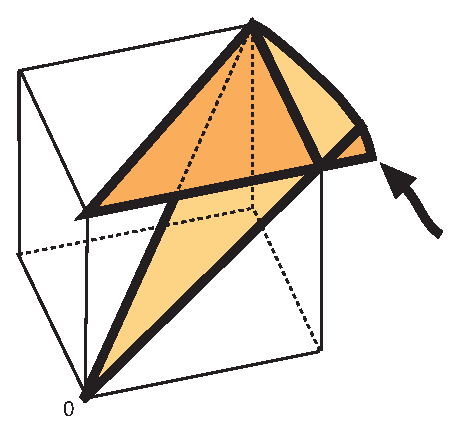
\includegraphics{\ps/quoin.eps}
  \caption{The quoin above a Rogers simplex is the part of the
  shaded solid outside
   the illustrated box.  It is bounded by the shaded planes, the plane through
   the front face of the box, and a sphere
   centered at the origin passing through the opposite corner of the box.}
  \label{fig:quoin}
\end{figure}

We let $\op{quovol}(a,b,c)$ be the volume of the
quoin.  As we will see in a moment, it depends only on $a,b,c$.

\begin{lemma}\label{lemma:quo-vol}
The volume $\op{quovol}(a,b,c)$ is given explicitly as follows
    \begin{equation}
    \begin{array}{lll}
    6\op{quovol}(a,b,c) &= (a+2c)  %
    % -(a^2+ac-2c^2)
    (c-a)^2\arctan(e)
        +a(b^2-a^2)e\\&-4c^3\arctan(e(b-a)/(b+c)),
    \label{eqn:3.3}
    \end{array}
    \end{equation}
where $e\ge0$ is given by $e^2(b^2-a^2)=(c^2-b^2)$.
%
 \index{quoin}
\end{lemma}

\begin{proof} We give the proof in some detail, because it illustrates
our method of calculating derived volumes from primitive volumes.
The calculations are essentially formal.

Let $\chi_X$ be the characteristic
function of $X$.  If $P = \chi_X$, write $\bar P$ for the characteristic
function of the complement of $X$.  We consider characteristic functions
only up to a null set, and this means that we can ignore issues such
as whether we take open half-spaces or closed half-spaces and so forth.

Set
$$
\begin{array}{lll}
  A &= \chi_X,\quad X = B(v_0,c)\\
  B &= \chi_X,\quad X = \op{aff}_+^0(\{v_0,v_1,v_2\},v_3)\\
  C &= \chi_X,\quad X = \op{aff}_-^0(\{v_1,p,p'\},v_0)\\
  D &= \chi_X,\quad X = \op{aff}_-^0(\{v_0,p,p'\},v_1)\\
  E &= \chi_X,\quad X = \op{aff}_+^0(\{v_0,v_1,p'\},p)\\
  F &= \chi_X,\quad X = SC(v_0,v_1,c,a/c)\\
\end{array}
$$

We see from Figure~\ref{fig:quo} that we have the following implications
$(f(x)=1)\implies (g(x)=1)$ when $f,g$ are any of the following characteristic
functions
  $$
   (f,g) = (B\bar C \bar D E,A),\quad
   (B\bar C E F,A),\quad (A B C D, E),\quad (A B C E,F).
  $$
(These implications are justified without pictures in Lemmas~\ref{XX}.)
%% XX Needed to add tarski calculations for these volumes.
We recognize $ABEF$ as the characteristic function $[SC]$ of a
conic cap, $B\bar C E F$ as the characteristic function $[WFR]$ of a
wedge of a frustum,  $AB\bar D E$ as the characteristic function $[ST]$
of a solid triangle, $B\bar C\bar D E$ as the characteristic function $[R]$
of a Rogers simplex.  The characteristic function $[Q]$
of the quoin is given
by $A B C D$.  We let $[X]$ be the characteristic function of
$A B C \bar D E$.

We then have formally that
$$
\begin{array}{lllll} \,[SC] &=  A B E F \\
     &= A B \bar C E F &+ A B C E F\\
     &= B \bar C E F &+ A B C D E F &+ A B C \bar D E F\\
     &= [WFR] &+ A B C D &+ A B C \bar D E\\
     &= [WFR] &+ [Q] &+ [X]\\ 
     \,[ST] &= A B \bar D E\\
     &= A B C \bar D E &+ A B \bar C \bar D E\\
     &= [X] &+ B \bar C \bar D E\\
     &= [X] &+ [R].
\end{array}
$$
Solving for $[Q]$, we get
\begin{equation}\label{eqn:qr}
  [Q] = [SC] - [WFR] + [R] - [ST].
\end{equation}
Thus, the volume of a quoin is expressed in terms of primitive volumes.
Substituting the given formulas for the volumes of primitives, we obtain
the result.  (It is necessary to use the Euler formula for solid
angle.)
\end{proof}

\begin{remark}  This type of analysis can be turned into an algorithm
for computing regions described by quadratic constraints in terms
of primitive volumes \cite{quad}.  All the volumes that arise in the
proof of the Kepler conjecture can be computed by this algorithm.
In particular, the proof of Lemma~\ref{lemma:quo-vol}.
\end{remark}

\begin{remark}  We can rewrite Equation~\ref{eqn:qr} as
$$
  [ST]-[R] = ([SC]-[WFR]) - [Q].
$$
That is, as we can see from Figure~\ref{def:quo}, the region
in a ball above and outside a Rogers simplex is the same as the
region in a ball above and outside a frustum and outside the quoin.
\end{remark}



\subsection{caps}

\begin{lemma}\label{lemma:cap-rogers}
Let $B(0,t)$ be a ball of radius $t$ centered at the origin.  Let
$v_1$ and $v_2$ be vertices.  Assume that $|v_1|< 2t$ and $|v_2|<2
t$.  Truncate the ball by cutting away the caps
   $$\op{cap}_i = \{x\in B(0,t) :  |x- v_i| < |x|\}.$$
Assume that the circumradius of the triangle $\{0,v_1,v_2\}$ is
less than $t$. Then the intersection of the caps, $\op{cap}_1\cap
\op{cap}_2$, is the union of four quoins.
\end{lemma}

\begin{proof} This is true by inspection.  See Figure~\ref{fig:capriquoin}.
Slice the intersection $\op{cap}_1\cap\op{cap}_2$ into four pieces
by two perpendicular planes: the plane through $\{0,v_1,v_2\}$,
and the plane perpendicular to the first and passing through $0$
and the circumcenter of $\{0,v_1,v_2\}$.  Each of the four pieces
is a quoin.
\end{proof}

\begin{figure}[htb]
  \centering
  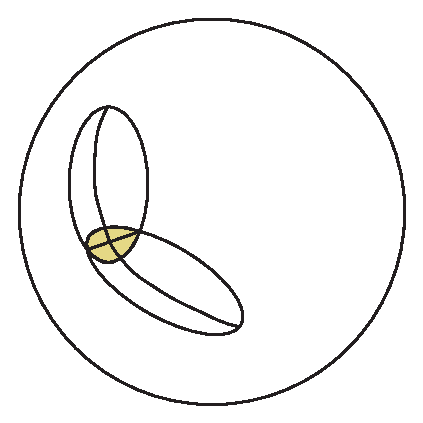
\includegraphics{\ps/capriquoin.eps}
  \caption{The intersection of two caps on the unit ball can
   be partitioned into four quoins (shaded).}
  \label{fig:capriquoin}
\end{figure}


\section{Truncated corner cells}\label{sec:tcc}
    %\oldlabel{4.10}

Let $S=(v_0,v,w_1,w_2)$ be a four-tuple of points in $\ring{R}^3$.  Assume
that $\{v_0,v,w_1,w_2\}$ is not coplanar.
We
attach a {\it corner cell} $CC(v_0,v,w_1,w_2,t,\lambda)$
to these four points and positive
real parameters $t,\lambda$.  Let $y=|v_0-v_1|$.  

Let $b=\eta(y,t,\lambda)$.
Construct the cone $C=\op{rcone}^0(v_0,v_1,\cos(\arc(y,t,\lambda)))$.
Let $P$ be the half-space containing $0$ bounded by
the perpendicular bisector of  $\{0,v\}$.
Let $C_1 = C\cap P \cap B(0,t_0)$.
Let $W$ be the wedge between $\op{aff}_+(\{0,v\},w_1)$ and
$\op{aff}_+(\{0,v\},w_2)$ formed by points 
   $$W = \{x\in\ring{R}^3 \mid 0< \azim(0,v,w_1,x) <
     \azim(0,v,w_1,w_2)\}.$$
Let $CC(v_0,v,w_1,w_2,t,\lambda) = C_1 \cap W$.

We also define a region $TC(v_0,v,w_1,w_2,t,\lambda)$ called
the {\it truncated corner cell}.  Let $b(v_0,v_1,w_i)$ be the
half-space containing $v_1$ that is bounded by the
plane passing through the origin and the
circumcenter of $\{v_0,v_1,w_i\}$ and that is perpendicular to the
plane $\op{aff}\{v_0,v_1,w_i\}$.  Set
  $$TC(v_0,v,w_1,w_2,t,\lambda) = CC(v_0,v,w_1,w_2,t,\lambda)
    \cap b(v_0,v_1,w_1)\cap b(v_0,v_1,w_2).$$ 
%% XX is there any potential back-wrap around problems with this
%% definition.  Do we want to intersect with the full b, or just the
%% forward part in W?


\subsection{Formulas for Truncated corner cells}\label{sec:ftcc}
    %\oldlabel{4.11}

We will assign a score to truncated corner cells, in such a way
that the score of the subcluster can be estimated from the scores
of the corner cells.

We write $C_0$ for a truncated corner cell.  We write $C_0^u$ for
the corresponding untruncated corner cell.  (Although we call this
the untruncated corner cell to distinguish it from the corner
cell, it is still truncated in the sense that it lies in the ball
at the origin of radius $t_0$.  It is untruncated in the sense
that it is not cut by the planes $(\ldots)^\perp$.)

For any solid body $X$, we define the {\it geometric} truncated
function by
    $$\vor_0^{g}(X) = 4(-\doct \op{vol}(X) + \sol(X)/3)$$
the counterpart for squander
    $$\tau_0^g(X) = \zeta\pt \sol(X) - \vor_0^g(X).$$
The solid angle is to be interpreted as the solid angle of the
cone formed by all rays from the origin through nonzero points of
$X$. We may apply these definitions to obtain formulas for
$\vor_0^{g}(C_0)$, and so forth.

The formula for the score of a truncated corner cell differs
slightly according to the convexity of the corner.  We start with
a convex corner $v$, and let $v_1$, $v$, and $v_2$ be consecutive
corners in the subregion.






Let $S=\{0,v,v_1,v_2\}$ be a simplex with $|v_1-v_2|\ge3.2$. The
formula for the score of a tcc $C_0(S)$ simplifies if the face of
$C_0$ cut by $\{0,v,v_1\}^\perp$ does not meet the face cut by
$\{0,v,v_2\}^\perp$. We make that assumption in this subsection.
Set
    $\chino(S) =\vor^g_0(C_0(S))$.

    $$
    \begin{array}{lll}
        \psi &= \arc(y_1,t_0,\lambda),\quad h=y_1/2,\\
        R'_{126}&=R(y_1/2,\eta_{126},y_1/(2\cos\psi)),
        \quad R_{126}=R(y_1/2,\eta_{126},t_0),\\
        \sol'(y_1,y_2,y_6) &= +\dih(R'_{126})(1-\cos\psi)-\sol(R'_{126}),\\
        \chino(S) &= \dih(S)(1-\cos\psi)\phi_0\\
            &\ -\sol'(y_1,y_2,y_6)\phi_0 -\sol'(y_1,y_3,y_5)\phi_0\\
            &\ +A(h)\dih(S)-
                4\doct (\quo(R_{126})+\quo(R_{135})).
    \end{array}
    $$
In the three lines giving the formula for $\chino$, the first line
represents the score of the cone before it is cut by the planes
$\{0,v,v_i\}^\perp$ and the perpendicular bisector of $\{0,v\}$.
The second line is the correction resulting from cutting the tcc
along the planes $\{0,v,v_i\}^\perp$. The face of the Rogers
simplex $R'_{126}$ lies along the plane $\{0,v,v_1\}^\perp$.  The
third line is the correction from slicing the tcc with the
perpendicular bisector of $\{0,v\}$.  This last term is the same
as the term appearing for a similar reason in the formula for
$\vor_0$ in Formula~\ref{eqn:3.7}. In this formula $R$ is the
usual Rogers simplex and $\quo(R_{ijk})$ is the quoin coming from
a Rogers simplex along the face with edges $(ijk)$.

The formula for the untruncated corner cell is obtained by setting
``$\sol'$'' and ``$\quo$'' to ``$0$'' in the expression for
$\chino$. Thus,
    $$
    \vor^g(C_0^u) = \dih(S)[(1-\cos\psi)\phi_0 + A(h)]
    $$
The formula depends only on $\lambda$, the dihedral angle, and the
height $|v|$.  We write $C_0^u = C_0^u(|v|,\dih)$, and suppress
$\lambda$ from the notation. The dependence on $\dih(S)$ is
linear:
    $$
    \tau^g_0(C_0^u(|v|,\dih))= (\dih/\pi)\tau^g_0(C_0^u(|v|,\pi)).
    $$

The dependence of $\chino$ on the fourth edge $y_4=|v_1-v_2|$
comes through a term proportional to $\dih(S)$.  Since the
dihedral angle is monotonic in $y_4$, so is $\chino$.  Thus, under
the assumption that $|v_1-v_2|\ge3.2$,  we obtain an upper bound
on $\chino$ at $y_4=3.2$. Our deformations will fix the lengths of
the other five variables, and monotonicity gives us the sixth.
Thus, the tccs lead to an upper bound on $\vor^g_0$ (and a lower
bound on $\tau^g_0$) that does not require interval arithmetic.


At a concave vertex, the formula is similar.  Replace
``$\dih(S)$'' with $``(2\pi-\dih(S))$'' in the given expression
for $\chino$. We add a superscript $-$ to the name of the function
at concave vertices, to denote this modification: $\chino^-(C_0)$.


\subsection{Formula for VC}


Let $S$ be a simplex and let $v$ be a vertex of that simplex. Let
$\op{VC}(S,v)$ be the subset of $|S|$ consisting of points closer
to $v$ than to any other vertex of $S$. By
Lemma~\ref{lemma:Q-divide}, if $S\in\CalQ_0(D)$, then
$$\op{VC}(S,0) = \op{VC}(D)\cap |S|.$$
Under the assumption that $S$ contains its circumcenter and that
every one of its faces contains its circumcenter, an explicit
formula for the volume $\op{vol}(\op{VC}(S,v))$ has been
calculated in \cite[Section~8.6.3]{part1}. This volume formula is
an algebraic function of the edge lengths of $S$, and may be
analytically continued to give a function of $S$ with chosen
vertex $v$:
  $$\op{vol}\,\op{VC}^\op{an}(S,v).$$



The following appeared as Claim~\ref{claim:volan}:
\begin{lemma}\label{lemma:volan}  %%Cf. claim:volan
Let $S=\{v_1,v_2,v_3,v_4\}$ be in the $\CalQ$-system. Then
    $$
    \sum_{i=1}^4 \op{volan}(S,v_i) = \sum_{i=1}^4
    \op{vol}(\op{VC}(S,v_i)) = \op{vol}(|S|).
    $$
\end{lemma}



 Let $S=\{v_0,v_1,v_2,v_3\}$ be a simplex. Fix $t$ in the range
$t_0\le t\le\sqrt2$.  Assume that $t$ is at most the circumradius
of $S$. Assume that it is at least the circumradius of each of the
faces of $S$.  Let $\op{VC}_t(S,v_0)$ be the intersection of
$\op{VC}(S,v_0)$ with the ball $B(v_0,t)$. Under the assumption
that $S$ contains its circumcenter and that every one of its faces
contains it circumcenter, an explicit formula for the volume
$$\op{vol}(\op{VC}_t(S,v_0))$$ is calculated by means of
Lemma~\ref{lemma:cap-rogers} through a process of inclusion and
exclusion. In detail, start with $|S|\cap B(v_0,t)$. Truncate this
solid by caps: $\op{cap}_1$, $\op{cap}_2$,\index{cap} and
$\op{cap}_3$ bounded by the sphere of radius $t$ centered at $v_0$
and the perpendicular bisectors (respectively) of $\{v_0,v_1\}$,
$\{v_0,v_1\}$, $\{v_0,v_2\}$.  If we subtract the volume of each
cap, $\op{cap}_i$, then we must add back the volume of the doubly
counted intersections of the caps.  The intersections of caps are
given as quoins (Lemma~\ref{lemma:cap-rogers}).  This leads to the
following formula. Let $h_i = |v_i|/2$ and
$\eta_{ij}=\eta(0,v_i,v_j)$, and let $S_3$ be the group of
permutations of $\{1,2,3\}$ in
\begin{equation}
   \op{vol}\,\op{VC}_t(S,v_0) =
   \sol(S)/3 - \sum_{i=1}^3 \frac{\dih(S,v_i)}{2\pi}\op{vol}\,\op{cap_i}
   +\sum_{(i,j,k)\in S_3} \quo(R(h_i,\eta_{ij},t)).
   \label{eqn:vol-theta-0}
\end{equation}


We extend Formula~\ref{eqn:vol-theta-0} by setting
    $$\quo(R(a,b,c)) = 0,$$
if the constraint $a < b < c$ fails to hold.  Similarly, set
$\op{vol}\,\op{cap}_i=0$ if $|v_i|\ge 2t$.  With these
conventions,  Formula~\ref{eqn:vol-theta-0} extends to all
simplices.  We write the extension of $\op{vol}\,\op{VC}_t(S,v)$
as
$$\op{vol}\,{\op{VC}^+_t}(S,v).$$


\subsection{Analytic continuation} %DCG 13.3, p144
    \oldlabel{5.3}

In this subsection we assume that $\lambda=1.6$ and that the
truncated corner cell under consideration lies at a convex vertex.

Assume that the face cut by $\{0,v,v_1\}^\perp$ meets the face cut by
$\{0,v,v_2\}^\perp$.  Let $c_i$ be the point on the plane
$\{0,v,v_i\}^\perp$ satisfying $|c_i-v|=1.6$, $|c_i|=t_0$. (Pick the root
within the wedge between $v_1$ and $v_2$.) The overlap of the two faces
is represented in Figure~\ref{fig:chi-anal-vs-geom}.

\begin{figure}[htb]
  \centering
  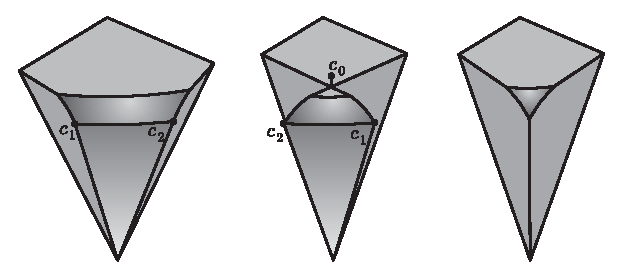
\includegraphics{\ps/samfigA54.eps}
  \caption{Different forms of truncated corner cells are shown.  The
  structure
  shown in the middle frame cannot occur.}
  \label{fig:chi-anal-vs-geom}
\end{figure}


We let $c_0$ be the point of height $t_0$ on the intersection of the
planes $\{0,v,v_1\}^\perp$ and $\{0,v,v_2\}^\perp$. We claim that $c_0$ lies
over the truncated spherical region of the tcc, rather than the wedges
of $t_0$-cones or the Rogers simplices along the faces $\{0,v,v_1\}$ and
$\{0,v,v_2\}$.  (This implies that $c_0$ cannot protrude beyond the corner
cell as depicted in the second frame of the figure.) To see the claim,
consider the tcc as a function of $y_4=|v_1-v_2|$. When $y_4$ is
sufficiently large the claim is certainly true.  Contract $y_4$ until
$c_0=c_0(y_4)$ meets the perpendicular bisector of $\{0,v\}$. Then $c_0$
is equidistant from $0,v,v_1$ and $v_2$ so it is the circumcenter of
$\{0,v,v_1,v_2\}$. It has distance $t_0$ from the origin, so the
circumradius is $t_0$. This implies that $y_4\le 2t_0$.

The tcc is defined by the constraints represented in the third
frame. The analytic continuation of the function
$\chino(S)=\chino^\anal(S)$, defined above, acquires a volume $X$,
counted with negative sign, lying under the spherical triangle
$(c_0,c_1,c_2)$. Extending our notation, we have an analytically
defined function $\chino^\anal$ and a geometrically defined function
$\chino^\geom$,
    $$
    \begin{array}{lll}
    \chino^\anal(S) &= \chino^\geom(S)-\op{c-vor}_0(X), \text{\ where}\\
    \op{c-vor}_0(X) &= 4(-\doct\op{vol}(X) +\sol(X)/3) = \phi_0\sol(X) <0.
    \end{array}
    $$
So $\chino^\anal >\chino^\geom$, and we may always use
$\chino(S)=\chino^\anal(S)$ as an upper bound on the score of a tcc.

For example, with $\lambda=1.6$ and $S = S(2.3,2.3,2.3,2.9,2,2)$, we
have
    $$\chino^\anal(S)\approx -0.103981, \quad\chino^\geom(S)\approx -0.105102.$$
Or, if $S=S(2,2,2t_0,3.2,2,2t_0)$, then
    $$\chino^\anal(S)\approx -0.0718957, \quad
    \chino^\geom(S)\approx -0.0726143.$$





\subsection{More on Truncated Corner Cells}

\begin{lemma}\label{lemma:tcc-est} 
 Let $C_0$ be a truncated corner cell with
parameter $\lambda=1.6$ and azimuth angle at least $\pi$. 
Then $\tau_0(C_0) > 0.297$.
\end{lemma}




\begin{proof}
 The Formula of Section~\ref{x-4.11}
gives
    $$
    \tau_0^g(C_0) =
    \tau^g_0(C^u_0(|v|,\dih))
    - \sol'(y_1,y_2,y_6) \phi'_0
    -\sol'(y_1,y_3,y_5)\phi'_0,
    $$
where $\phi'_0 = \zeta\pt-\phi_0 < 0.6671$. (The conditions $y_5\ge3.07$
and $y_6\ge 3.07$ force the faces along the these edges to have
circumradius greater than $t_0$, and this causes the ``$\quo$'' terms in
the formula to be zero.)

By monotonicity in $\dih$, a lower bound on $\tau^g_0(C^u_0)$ is
obtained at $\dih=\pi$. $\tau_0(C^u_0(|v|,\pi))$ is an explicit monotone
decreasing rational function of $|v|\in[2,2t_0]$, which is minimized for
$|v|=2t_0$.  We find
    $$\tau_0(C_0^u(|v|,\dih))\ge\tau_0(C_0^u(2t_0,\pi)) >0.32.$$

The term $\sol'(y_1,y_3,y_5)$ is maximized when $y_3=2t_0$, $y_5=3.07$,
so that $\sol'< 0.017$.  (This was checked with interval arithmetic in
Mathematica.) Thus,
    $$\tau_0(C_0(v))\ge 0.32 - 2(0.017) \phi_0' > 0.297.$$
\end{proof}



\begin{lemma}  Let $C^u_0(y,\azim)$ be an untruncated corner
cell with parameter 1.815, $2\le y\le 2.2$, 
and azimuth angle at least $\pi$.  Then
 $$\tau_0(C^u_0(2.51,\pi))-\maxpi > \squander.$$
\end{lemma}

\begin{proof}
This is an explicit monotone decreasing rational function of one
variable. The minimum, which occurs at $h=2.51$, is
    $$\tau_0(C^u_0(2t_0,\pi))-\maxpi > \squander.$$
\end{proof}

\begin{lemma}\label{lemma:2tcc} 
Let $C_1$ and $C_2$ be untruncated corner cells, both
with azimuth angle at least $\pi$ and parameter $\lambda=1.945$.
Suppose that $C_1$ is along $\{0,v_1\}$ and $C_2$ is along
$\{0,v_2\}$, with $|v_1-v_2|\ge 3.2$.  Suppose that
$2\le |v_i|\le 2.51$, for $i=1,2$.  Then
$\tau_0(C_1\cup C_2) > \squander + \maxpi$.
\end{lemma}

\begin{proof}
Suppose first that $C_1$ and $C_2$ are disjoint.
As in the previous lemma, when $\lambda=1.945$, a lower bound on
what is squandered by the corner cell is obtained for  $|v|=2t_0$,
$\dih=\pi$. The explicit formulas give penalty-free squander
$>0.734$ for each. Two disjoint corner cells give
squander $ 2(0.734) >\squander +\maxpi$.  
Suppose two at $v_1,v_2$ meet at an
interior point. The lowest bound is obtained when $|v_1-v_2|=3.2$,
the shortest distance possible.

We define a function $f(y_1,y_2)$ that measures what the union of the
overlapping corner cells squander.  Set $y_i = |v_i|$, $\ell=3.2$, and
    $$
    \begin{array}{lll}
    \alpha_1 &= \dih(y_1,t_0,y_2,\lambda,\ell,\lambda),\\
    \alpha_2 &= \dih(y_2,t_0,y_1,\lambda,\ell,\lambda),\\
    \sol &= \sol(y_2,t_0,y_1,\lambda,\ell,\lambda),\\
    \phi_i &= \phi(y_i/2,t_0),\quad i=1,2,\\
    \lambda&=3.2-t_0=1.945,\\
    f(y_1,y_2)&=
    2(\zeta\pt-\phi_0)\sol+
    2\sum_1^2 \alpha_i(1-y_i/(2t_0))(\phi_0-\phi_i)\\
        &\quad +\sum_1^2 \tau_0(C(y_i,\lambda,\pi-2\alpha_i)).
    \end{array}
    $$
An interval calculation\footnote{\calc{984628285}} %A14
gives $f(y_1,y_2)>\squander+\maxpi$, for $y_1,y_2\in[2,2t_0]$.
\end{proof}




\section{Scores}
\label{sec:ssc}

The last section introduced a function $\sigma$ called the score.
We show that the function $\sigma$ can be expressed as a sum over
terms attached to each of the standard regions.

\begin{definition} \label{def:standard-cluster}
A {\it standard cluster\/} is a pair $(R,D)$ where $D$ is a
centered packing and $R$ is one of its standard regions.  A {\it
quad cluster\/} is the standard cluster obtained when the standard
region is a quadrilateral.
\end{definition}
%
 \index{cluster!standard}
 \index{cluster!quad}
 \index{quad cluster}

%Recall $|S|$ is the convex hull of a set $S\subset
%\ring{R}^3$.

We break $\sigma$ into a sum
   \begin{equation}
   \sigma(D) = \sum_R\,\sigma_R(D),
   \end{equation}
indexed by the standard clusters $(R,D)$.  Let
   $$
   \op{VC}_R(D) = \op{VC}(D)\cap \op{cone}(R),
   $$
whenever $R$ is a measurable subset of the unit sphere.  Let
   $$
   \CalQ_0(R,D) = \{Q\in \CalQ_0(D) : Q\subset \op{cone}(R)\}.
   $$
By Lemma~\ref{lemma:Q-in-region},
 each $Q$ is entirely contained in the cone over a single
standard region.

\begin{definition} \label{def:score-std-region}
   Let $R$ be a measurable subset of the unit sphere.  Set
      $$
      \vor_R(D) =4\left(-\doct \op{vol}\,\op{VC}_R(D)  +
      \sol(R)/3\right).
      $$
      Let $R$ be a standard region. Set
      $$
      \sigma_R(D) = \vor_R(D) - 4\doct
         \sum_{Q\in\CalQ_0(R,D)} A_1(Q,c(Q,D),0).
      $$
\index{vzorR@$\vor_R$} \index{zzsigmaR@$\sigma_R$}
\end{definition}

\begin{lemma} $\sigma(D) = \sum_R\sigma_R(D)$, where the sum runs
over all standard regions $R$.
\end{lemma}

\begin{proof}
   $$
   \begin{array}{lll}
      \sigma(D)
      &= -4\doct (\op{vol}\,\Omega(D) + A_0(D))+16\pi/3\\
      &= -4\doct (\op{vol}\,\op{VC}(D)+\sum_{Q\in\CalQ_0(D)}
         A_1(Q,c(Q,D),0)) + (4) (4\pi/3)\\
      &= \sum_R 4\left (-\doct \op{vol}\,\op{VC}_R(D) -\doct
         \sum_{Q\in\CalQ_0(R,D)} A_1(Q,c(Q,D),0) +
         \sol(R)/3\right).
   \end{array}
   $$
\end{proof}

Also, we have
    \begin{equation}
    \op{vor}(D)=\sum_{R\in \CalR(D)}
    \op{vor}_R(D).
    \label{eqn:vorD}
    \end{equation}

\begin{lemma}\label{lemma:R'}
Let $R'\subset R$ be the part of a standard region that does not
lie in any cone over any $Q\in Q_0(R,D)$.  Then
   $$
   \sigma_R(D) = \vor_{R'}(D)
      + \sum_{Q\in\CalQ_0(R,D)} \sigma(Q,c(Q,D),0).
   $$
\end{lemma}

\begin{proof} Substitute the definition of $A_1$
(Equation~\ref{eqn:a1-sigma}) into the definition of
$\sigma_R(D)$, noting that $\op{VC}(Q,0) = \op{VC}_{R''}(D)$,
where $R''$ is the intersection of $Q$ with the unit sphere.
\end{proof}

\begin{remark}   Lemma~\ref{lemma:R'} explains why we have chosen
the same symbol $\sigma$ for the functions $\sigma_R(D)$ and
$\sigma(Q,c,v)$.  We can view Lemma~\ref{lemma:R'} as asserting a
linear relation in the functions $\sigma$:
   $$\sigma_R(D) = \sigma_{R'}(D) + \sum \sigma(Q,c,0).$$
The sum runs over $Q\in\CalQ_0$ that lie in the cone over $R$.
\end{remark}

\section{Scores of Simplices and Cones}

Many of the functions in this paper are defined by terms involving
volumes of simple solids.  To give estimates on the functions, it
is often convenient to partition the solids into smaller pieces
and then define corresponding functions on each of the pieces. For
this reason, we define some variants of the functions $\vor$ and
$\sigma$.

\begin{remark}\label{remark:vor}\index{vor}\index{c-vor}\index{score}
We now define a few more variants of the function $\vor$. The
function $\svor$ and its truncated version  $\svor(\cdot,t)$ have
been defined already. The function $\vor_R(D)$ will also be given
a truncated version $\vor_R(D,t)$, for a real truncation parameter
$t\ge 0$. The special case, $\vor_R(D,t_0)$ will be abbreviated
$\vor_{0,R}(D)$. There will be another variant $\op{r-vor}$ for
Rogers simplices, and another $\op{c-vor}$ for general sets.  The
general form of these functions is
    $$\op{c-vor}(X) = 4 (-\doct\op{vol}(X) + \sol(X)/3),$$
for any subset $X\subset \ring{R}^3$.   The differences between
the different versions of $\vor$ come from the different choices
of the set $X$ and the way they are parametrized.
\end{remark}

\begin{definition}  \label{def:r-vor}\index{r-vor}
Let $R=R(a,b,c)$ be a Rogers simplex. Assume that the vertex
terminating the edges of lengths $a$, $b$, and $c$ is situated at
the origin. Let
    $$\op{r-vor}(R) = 4 (-\doct\op{vol}(R) + \sol(R)/3).$$
\end{definition}

\begin{definition}\label{def:cone}
 Let $C(h,t)$ denote the compact cone of height $h$
and circular base. Set
%of area $\pi(t^2-h^2)$. Set
    $$
    \phi(h,t)=2(2-\doct  t h (h+t))/3.
    $$
\index{right circular cone}\index{cone}
 Then
    \begin{equation}
    \op{c-vor}(C(h,t))=2\pi(1-h/t)\phi(h,t).
    \label{eqn:3.2}
    \end{equation}
 \end{definition}


\begin{remark}\label{remark:score}
Below, we introduce variants of the function $\sigma$. We have
already encountered $\sigma$ in Definitions~\ref{def:sigma},
\ref{def:score}, and \ref{def:score-std-region}. Informally, we
call $\sigma$ (and various functions that are closely related to
it) the {\it score}. Equation~\ref{eqn:3.2} represents the {\it
score\/} of $C(h,t)$. The solid angle of $C(h,t)$ is
$2\pi(1-h/t)$, so $\phi(h,t)$ is the score per unit area. Also,
$\phi(t,t)$ is the score per unit area of a ball of radius $t$.
That is, $\phi(t,t) = 4(-\doct\op{vol}/\sol + 1/3)$.\index{score}
\end{remark}


We set
    \begin{equation}
    \begin{array}{lll}
    \svor(S,t) &=
    \sol(S)\phi(t,t)
    +\sum_{i=1,\ h_i\le t}^3 d_i (1-h_i/t) (\phi(h_i,t)-
    \phi(t,t)) \\
    &-\sum_{(i,j,k)\in S_3}
    4\doct
    \quo(R(h_i,\eta(y_i,y_j,y_{k+3}),t)).
    \label{eqn:3.5}
    \end{array}
    \end{equation}
In the definition, we adopt the convention that $\quo(R)=0$, if
$R=R(a,b,c)$ does not exist (that is, if the condition
    $0< a\le b\le c$
is violated). In the second sum, $S_3$ is the set of permutations
on three letters. This definition is compatible with
Definition~\ref{def:svor}.

Similarly, we define $\vor_P(D,t)$ for arbitrary standard clusters
$(P,D)$.  (We shift notation from $R$ to $P$ for a standard region
to avoid conflict with Rogers simplices $R$ in the following
definition.)  Extending the notation in an obvious way, we have
    \begin{equation}
    \begin{array}{lll}
    \vor_P(D,t) &=
    \sol(P)\phi(t,t)
    +\sum_{|v_i|\le 2t} d_i (1-|v_i|/(2t)) (\phi(|v_i|/2,t)-
    \phi(t,t)) \\
    &-\sum_{R} 4\doct \quo(R).
    \label{eqn:3.7}
    \end{array}
    \end{equation}
The first sum runs over vertices in $P$ of height at most $2t$.
The second sum runs over Rogers simplices $R(|v_i|/2,\eta(F),t)$
in $P$, where $F=\{0,v_1,v_2\}$ is a face of circumradius
$\eta(F)$ at most $t$, formed by vertices in $P$.  The constant
$d_i$ is the total dihedral angle along $\{0,v_i\}$ of the
standard cluster. The truncations $t=t_0=1.255$ and $t=\sqrt2$
will be of particular importance.
    Set $A(h) = (1-h/t_0) (\phi(h,t_0)-\phi(t_0,t_0))$.\index{A}

\begin{remark}  We have introduced both untruncated and truncated
versions of functions $\vor$ and $\sigma$.  The truncated versions
are used to give upper bounds on the untruncated versions.  For
example,  in the function $\sigma(D)$, the $V$-cell contributes
through its volume, as in Remark~\ref{remark:vor}.  The volume
appears with a negative coefficient $-4\doct$.  Thus, we obtain an
upper bound on $\sigma(D)$ by discarding bits of volume from the
$V$-cell.   This suggests that we might try to give upper bounds
on the score $\sigma(D)$ by truncating the $V$-cell in various
ways. This is the reason for the truncated versions of these
functions.
\end{remark}

\begin{lemma}\label{lemma:Zcount}
    For all $p\in\ring{R}^3$ and all $r\ge 0$, the set
    $\ring{Z}^3\cap B(p,r)$ is finite of cardinality at most
    $4\pi (r+\sqrt3)^3/3$.
\end{lemma}

\begin{proof}  If $v\in\ring{Z}^3\cap B(p,r)$, then the ith
coordinate $v_i$ of $v$ must lie in the finite range
    $$
    p_i - r \le v_i \le p_i + r.
    $$
Hence there are only finitely many possibilities for $v$.


Place an open unit cube at each point of $\ring{Z}^3\cap B(p,r)$.
The cubes are measurable, disjoint, and contained in
$B(p,r+\sqrt3)$.  Thus, the combined volume of the cubes, which is
$|\ring{Z}^3\cap B(p,r)|$,  is no greater than the volume of the
containing ball.  The result follows.
\end{proof}

\begin{lemma}\label{lemma:Zlow-count}
  For all $p\in\ring{R}^3$ and all $r\ge\sqrt3$, the set
    $\ring{Z}^3\cap B(p,r)$ is finite of cardinality at least
    $4\pi (r-\sqrt3)^3/3$.
\end{lemma}

\begin{proof} We have already established finiteness in
Lemma~\ref{lemma:Zcount}.  Place a closed unit cube at each point
of $\ring{Z}^3\cap B(p,r)$.  The cubes are measurable and cover
$B(p,r-\sqrt3)$.  Thus, the combined volume of the cubes is at
least the volume of the covered ball.  The result follows.
\end{proof}

\begin{lemma}\label{lemma:Zr2}
For all $p\in\ring{R}^3$, and $k,k'>0$, there exists a $C$ such
that for all $r\ge k'$, we have
    $$
    \ring{Z}^3 \cap (B(p,r+k) \setminus B(p,r-k')) \le C r^2.
    $$
\end{lemma}

\begin{proof}  When $r \ge k'+\sqrt3$, the previous two lemmas show
that the cardinality is at most $4\pi/3$ times
    $$(r + \sqrt3)^3 - (r - \sqrt3)^3 \le C' r^2$$
for some $C'$.  Similarly, if $k'\le r\le k'+\sqrt3$, the
cardinality is at most some fixed constant $C''$.  The result
easily follows.
\end{proof}



%\section{The Function K}
%\label{sec:K} %DCG p105-106.
%% No longer used.  Proof of -1.04 lemma was rewritten.
%%
%
%We define a function $K(S)$ on
%certain simplices $S$ with circumradius at least $\sqr2$. Let
%$S=S(y_1,y_2,\ldots,y_6)$.  Let $R(a,b,c)$ denote a Rogers
%simplex. Set
%    \begin{equation}
%    K(S) = K_0(y_1,y_2,y_6)+K_0(y_1,y_3,y_5)
%    + \dih(S)(1-y_1/\sqr8) \phi(y_1/2,\sqr2),
%    \label{eqn:KS}
%    \end{equation}
%where
%    $$
%    \begin{array}{lll}
%    K_0(y_1,y_2,y_6) &= \op{r-vor}(R(y_1/2,\eta(y_1,y_2,y_6),\sqr2))
%        +\op{r-vor}(R(y_2/2,\eta(y_1,y_2,y_6),\sqr2))\\
%        &- \dih(R(y_1/2,\eta(y_1,y_2,y_6),\sqr2))
%        (1-y_1/\sqr8)\phi(y_1/2,\sqr2).
%    \end{array}
%    $$
%(If the given Rogers simplices do not exist because the condition
%$0<a<b<c$ is violated, we set the corresponding terms in these
%expressions to 0.) The function $K(S)$ represents the part of the
%score coming from the four Rogers simplices along two of the faces
%of $S$, and the conic region extending out to $\sqr2$ between the
%two Rogers simplices along the edge $y_1$ (Figure~\ref{fig:KS}).
%This region is closely related to the regions $\BigD(v,W)$ of
%Definition~\ref{def:delta-e}, with the difference that the regions
%$\BigD$ lie in a ball of radius $\eta_0(|v|/2)$, but the regions
%here are truncated at $\sqrt2$.
%
%\begin{figure}[htb]
%  \centering
%  \includegraphics{\ps/diag43.ps}
%  \caption{The set measured by the function $K(S)$.}
%  \label{fig:KS}
%\end{figure}
%
%

\section{The Function anc}
\label{sec:anc} %DCG p 107.

Set $\phi_0=\phi(t_0,t_0)\approx -0.5666$. We define
    \begin{equation}\cro(h) =
2\pi(1-h/\eta_0(h))(\phi(h,\eta_0(h))-\phi_0). \end{equation} It
is equal to $-4\doct$ times the volume of the region outside the
sphere of radius $t_0$ and inside the finite cone
$C(h,\eta_0(h))$.  If $v$ is an enclosed vertex of height
$2h\in[2t_0,\sqr8$],
 such that every other vertex $v'$ of the
standard cluster satisfies
$$\eta(|v|,|v'|,|v-v'|)\ge \eta_0(h),$$ then the
solid represented by $\cro(|v|/2)$ lies outside the truncated
$V$-cell, but inside the $V$-cell, so that if $P$ is a quad
cluster,
 $$\op{c-vor}(V_P) < \op{c-vor}_0(V_P) + \cro(|v|/2).$$
If a vertex $v'$ satisfies $\eta(|v|,|v'|,|v-v'|)\le\eta_0(h)$,
then by the monotonicity of the circumradius of acute triangles,
$v'$ is an anchor of $v$.  This anchor clips the crown just
defined, and we add a correction term $\anc(|v'|,|v|,|v-v'|)$ to
account for this. Figure~\ref{fig:anchor} illustrates the terms in
the definition of $\anc()$.



\begin{figure}[htb]
  \centering
  \includegraphics{\ps/diag44.ps}
  \caption{An illustration of the terms $\anc$.}
  \label{fig:anchor}
\end{figure}


Set
    \begin{equation}
    \begin{array}{lll}
    \anc(y_1,y_2,y_6) &= -\dih(R_1)\cro(y_1/2)/(2\pi)
        -\sol(R_1)\phi_0+\op{r-vor}(R_1)\\
    &-\dih(R_2)(1-y_2/2t_0)(\phi(y_2/2,t_0)-\phi_0)
        -\sol(R_2)\phi_0 + \op{r-vor}(R_2),
    \label{eqn:4.5}
    \end{array}
    \end{equation}\index{anc@$\anc$}
where $R_i=R(y_i/2,\eta(y_1,y_2,y_6),\eta_0(y_1/2))$, for $i=1,2$.
In general, there are Rogers simplices on both sides of the face
$\{0,v,v')$, and this gives a factor of 2. For example, if $v$ has
a single anchor $v'$, then
$$\op{c-vor}(V_P) < \op{c-vor}_0(V_P) + \cro(|v|/2) + 2\anc(|v|,|v'|,|v-v'|).$$
However, if the anchor gives a face of an upright quarter, only
one side of the face lies in the $V$-cell,
 so that the factor of 2 is not required.
For example, $v'$ has context $\x(2,1)$ with upright quarter $Q$,
and if there are no other enclosed vertices, and if $v',v''$ are
the anchors along the faces of the quarter,  then
    $$
    \begin{array}{lll}
    \op{c-vor}(V_P)&< \op{c-vor}_0(V_P) +(1-\dih(Q)/(2\pi))\cro(|v|/2)\\
    &+\anc(|v|,|v'|,|v-v'|)+\anc(|v|,|v''|,|v-v''|).
    \end{array}
    $$
In general, when there are multiple anchors around the same
enclosed vertex $v$, we add a term $(2-k)\anc$ for each anchor,
where $k\in\{0,1,2\}$ is the number of quarters bounded by the
face formed by the anchor. We must be cautious (see
Condition~\ref{enum:wedge2} in Definition~\ref{def:wedge} in the
use of this formula. If the circumradius of $\{0,v,v',v''\}$ is
less than $\eta_0(|v|/2)$, the Rogers simplices used to define the
terms $\anc()$ at $v'$ and $v''$ overlap. When this occurs, the
geometric decomposition on which the correction terms $\anc()$ are
based is no longer valid. In this case, other methods must be
used.

\begin{figure}[htb]
  \centering
  \includegraphics{\ps/diag46.ps}
  \caption{The terms $\anc$ near an upright quarter.}
  \label{fig:anchor-quarter:bis}
\end{figure}


%% Moved from DCG 11.2 Contexts.
Crowns and anchor correction terms are used in Section~\ref{sec:bounds}
to erase upright quarters.  We imitate those methods here. The functions
$\cro$ and $\anc$ are defined and discussed in Section~\ref{sec:bounds}.
If
    $S=S(y_1,\ldots,y_6)$
is a simplex along $\{0,v\}$, set
    $$\kappa(S(y_1,\ldots,y_6))=\cro(y_1/2)\dih(S)/(2\pi) +
        \anc(y_1,y_2,y_6)+\anc(y_1,y_3,y_5).
    $$
$\kappa(S)$ is a bound on the difference in the score resulting from
truncation around $v$. Assume that $S$ is the simplex formed by $\{0,v\}$
and two consecutive anchors $\{v_1,v_2\}$ around $\{0,v\}$. Assume further that the
circumradius of $S$ is at least $\eta_0(y_1/2)$.  Then we have
    $$\kappa(S) = -4\doct \op{vol}(\bigd(v,W)),$$
with $\bigd$ given in 
Definition~\ref{def:delta-e}. To see this, it is a matter of interpreting
the terms in $\kappa$. The function {\it crown\/} enters the volume
through the region over the spherical cap $D_0$ of
Section~\ref{sec:deltaP}, lying outside $B(t_0)$.  By multiplying by
$\dih(S)/(2\pi)$, we select the part of the spherical cap over the
wedge $W$ between the anchors.  The terms {\it anc\/} adjust
for the four Rogers simplices that enter the construction.


